% !TeX root = thesis.tex

\chapter{Evaluation}
\label{ch:evaluation}
This chapter will evaluate the performance of framework presented in the previous chapter. In the first section, the two test subjects that will be used in the subsequent experiments will be introduced. The next section will restate the research questions formally, and extend these. Afterwards, the procedure of how the data was obtained will be elaborated. The final section will provide answers to the research questions as well as present the results of applying \tcp{} to the test subjects.

% !TeX root = ../thesis.tex

\section{Test subjects}

\subsection{Dodona}
Dodona\footnote{\url{https://dodona.ugent.be/}} is an open source online learning environment created by Ghent University, allowing students from secondary schools and universities in Belgium and South-Korea to submit solutions to programming exercises and receive automated feedback. The application is built using the Ruby-on-Rails web framework. In order to automate the testing process of the application, Dodona makes use of Github Actions (\autoref{sssec:github-actions}) to run tests using the default \texttt{MiniTest} testing framework. The coverage of the test suite is being recorded by \texttt{SimpleCov}\footnote{\url{https://github.com/colszowka/simplecov}}.

\subsection{Stratego}
Leg uit wat het is.
% !TeX root = ../thesis.tex

\section{Research questions}
We will answer the following research questions in the subsequent sections:

\paragraph*{RQ1: What is the probability that a test run will contain at least one failed test case?}
The first research question will provide useful insights into whether a typical test run tends to fail or not. The expectancy is that the probability of failure will be rather low, indicating that it is not strictly necessary to execute every test case and therefore making a case for \tsm{}.

\paragraph*{RQ2: What is the average duration of a test run?}
Measuring how long it takes to execute a typical test run is required to estimate the benefit of applying any form of test suite optimisation. We will only consider successful test runs, to reduce bias introduced by prematurely aborting the execution.

\paragraph*{RQ3: Suppose that a test run has failed, what is the probability that the next run will fail as well?}
The ROCKET algorithm (\cref{ssec:alg-rocket}) relies on the assumption that if a test case has failed in a given test run, it is likely to fail in the subsequent run as well. This research question will investigate the correctness of this hypothesis.

\paragraph*{RQ4: How can \tcp{} be applied to Dodona and what is the resulting performance benefit?}
This research question will investigate the possibility to apply the \velocity{} framework to the Dodona project and analyse how quickly the available predictors can discover a failing test case.

\paragraph*{RQ5: Can the Java agent be applied to Stratego?}
Since the testing framework used by Stratego should be supported natively by the Java agent, this research question will verify its compatibility. Furthermore, we will analyse the prediction performance, albeit with a small number of relevant test runs.
% !TeX root = ../thesis.tex

\section{Data collection}\label{sec:eval-data}

\subsection{\travisci{} build data}
In order to answer the first three research questions, build data for several projects hosted on \travisci{} (\autoref{sssec:travisci}) was used. This data was obtained from two sources.\\

\noindent The first source is a database of \SI{35793144} jobs, provided by Durieux et al \cite{travisanalysis}. Due to the magnitude of this dataset (\SI{61.11}{\gibi\byte}), a big data framework is required to parse the log files. In order to collect the required data for the three first research questions, three MapReduce pipelines have been created using the Apache Spark\footnote{\url{https://spark.apache.org/}} framework.\\



\noindent Additionally, another \SI{3702595} jobs have been analysed from the \emph{TravisTorrent} project. This project \cite{msr17challenge} scrapes the API of \travisci{} and combines this with data obtained from the GitHub API to infer additional information about the test run, such as the programming language and the amount of failed test cases. The creators of TravisTorrent have provided a Google BigQuery\footnote{\url{https://bigquery.cloud.google.com/}} interface to allow querying the dataset. The following queries have been executed:

\subsection{Dodona build data}
// bespreek dodona instrumenter.
\clearpage
% !TeX root = ../thesis.tex

\section{Results}

\subsection{RQ1: Probability of failure}\label{ssec:results-rq1}
\autoref{fig:rq1-failure-probability} contains two pie charts that illustrate the amount of failed and successful test runs. The left chart contains the results of the dataset provided by Durieux et al \cite{travisanalysis}. This dataset contains $\SI{4558279}{}$ failed test runs versus $\SI{24323724}{}$ successful runs, which corresponds to a failure probability of $\SI{18.74}{\percent}$. The other pie chart visualises data from the TravisTorrent project. According to this dataset, the run has failed prior to starting the test suite in $\SI{42.89}{\percent}$ of the executions. For the remaining part of the runs, $\SI{225766}{}$ out of $\SI{2114920}{}$ executions contained at least one failed test case, corresponding to a failure percentage of $\SI{10.67}{\percent}$.

\begin{figure}[htbp!]
	\centering
	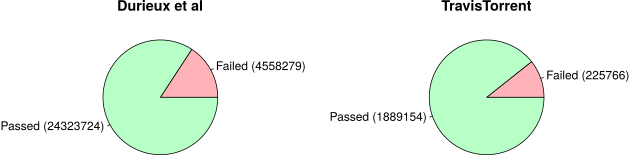
\includegraphics[width=\textwidth]{assets/charts/rq1-failure-probability.pdf}
	\caption{Probability of test run failure}
	\label{fig:rq1-failure-probability}
\end{figure}

\subsection{RQ2: Probability of consecutive failure}
In order to find consecutive failures, only the TravisTorrent project can be used as every entry in this dataset contains the identifier of the previous build which is required to link consecutive builds. The dataset contains $\SI{211040}{}$ test runs of which the test suite of the preceding test run was both executed and contained at least one failed test case. As illustrated in \autoref{fig:rq2-consecutive-failure}, $\SI{109224}{}$ of these test runs failed as well, versus $\SI{101816}{}$ test runs ($\SI{51.76}{\percent}$) that did succeed.

\begin{figure}[htbp!]
	\centering
	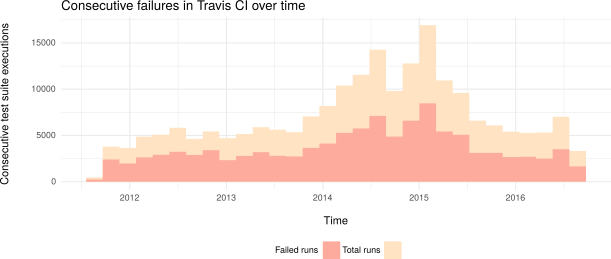
\includegraphics[width=\textwidth]{assets/charts/rq2-consecutive-failure.pdf}
	\caption{Consecutive test run failures on \travisci{}}
	\label{fig:rq2-consecutive-failure}
\end{figure}

\subsection{RQ3: Average test run duration}

maak boxplot van 5.3

- tests lager dan 10 seconden werden genegeerd aangezien dit een failure in de setup betekent.
- de zeer lange tests maken gebruik van mutation testing
- gegroepeerd per hoeveelheid en genormaliseerd op de y-as


\subsection{RQ4: Applying \tcp{} to Dodona}

voor 5.4:

- duration per run
- failed test cases per run
- time (ms) until first failed test case
- time (ms) until first prioritised failed test case